\documentclass[a4paper,10pt]{article}
%\documentclass[a4paper,10pt]{scrartcl}

\usepackage[utf8]{inputenc}
\usepackage{graphicx}
\usepackage{float}
\usepackage{anysize}

\marginsize{2cm}{2cm}{1cm}{1cm}
\title{Documentación de los programas, tarea 1 elo329.}
\author{Pascal Ernesto Sigel Olivares}
\date{abril-2014}

\pdfinfo{%
  /Title    (Documentación tarea 1 de Programación orientada a objetos UTFSM, 2014 Semestre 1)
  /Author   (Pascal Ernesto Sigel Olivares)
  /Creator  (Pascal Ernesto Sigel Olivares)
  /Producer ()
  /Subject  ()
  /Keywords (Programación orientada a objetos, POO, UTFSM, elo329, Simulación de experimentos simples, simulación)
}

\begin{document}
\maketitle
\newpage
\section{Introducción:}


En el presente documento se explicará cada uno de los programas los cuales están cada uno en su carpeta personal llamada etapa(n) donde n 
es un número. El proyecto está separado en varias etapas, desde la número 1 hasta la número 5 y cada etapa agrega alguna característica a 
la anterior.\newline

El proyecto en sí es un simulador de interacciones físicas como, por ejemplo, el choque de dos bolas, una bola junto con un resorte 
o un bloque con rose con bolas y resortes en cualquier disposición deseada.\newline

En la próxima sección se mostrarán algunos detalles importantes de el programa etapa1, que consta de dos bolas una en resposo y la otra en 
movimiento que chocan con choque elástico.

\section{Etapa 1}

El programa etapa 1 es la primera versión de este simulador el cual simula la interacción de dos bolas que chocan. 
En este programa se crea la primera versión del simulador con las clases PhysicsLab,MyWorld, PhysicsElement y Ball. Se hará
una descripción de cada una de estas clases.\newline

\subsection{Clase PhysicsLab:}


La clase PhysicsLab es la clase main del proyecto, esta clase manipula el objeto de tipo MyWorld creándolo y dándole los elementos que
interaccionarán en este ``mundo'' simulado.\newline

\subsection{Clase MyWorld:}


Esta clase es la que maneja la interacción entre los elementos del mundo simulado, el método principal de esta clase es el método \textbf{simulate}
el cual comienza la simulación. En la función \textbf{simulate} 
se requiere que cada elemento físico (PhysycsElement) sea capaz de calcular su próximo estado.\newline

\subsection{PhysicsElement:}


Los elementos físicos son una clase abstracta de la cual nacen los elementos como bolas, resores, bloques y cualquier otro elemento físico.\newline

\subsection{Ball:}


Esta clase se extiende (desciende) de la clase PhysicsElement y representa una bola la cual tiene masa, velocidad y posicion. En esta clase 
se calcula el próximo estado.\newline


\subsection{Experimento y resultados:}

Lease el archivo README para ejecutar el programa.\newline

El caso ha simular puede ser representado con la siguiente figura:

\begin{figure}[H]
 \centering
 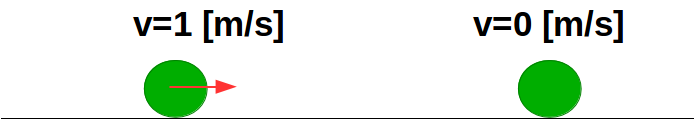
\includegraphics[scale=0.3]{./FigureA.png}
 \caption{Simulación realizada en etapa 1, en la simulación la posición inicial de la bola con velocidad es x=1[mts] y la otra es en x=2.56[mts] ambos con radio 0.1 [mts].}
  \label{etapa1.1}
\end{figure}


Se ha simulado la situación descrita en la figura \ref{etapa1.1}, o sea el choque elástico entre dos
bolas, con la simulación se obtuvieron el siguiente gráfico.

\begin{figure}[H]
 \centering
 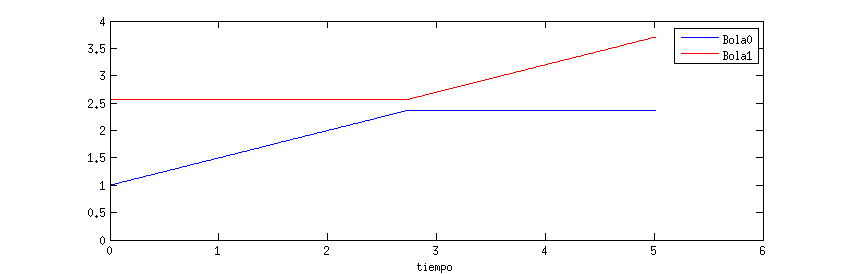
\includegraphics[scale=0.5]{./simulacion_etapa1.png}
 \caption{Resultados simulación etapa 1, Bola 0: bola inicialmente en movimiento y Bola 1: vola inicialmente en reposo.}
  \label{etapa1.2}
\end{figure}

Como se observa en el gráfico de la figura \ref{etapa1.2} cuando la bola 0 colisiona con la bola 1 (a 0.2 mts de distancia dado sus radios) 
la bola 1 obtiene todo el movimiento como se esperaría de un choque elástico de dos masas iguales y una en reposo.\newline

\subsection{Problemas que ocurrieron:}

\subsubsection{Problema con formatos:}


Por defecto Java usa el formato de numeros flotantes con coma ``,'' pero software como matlab usan el formato flotante con punto ``.''
Por lo que en vez de usar \textbf{System.out.print()} se usó \textbf{System.out.format(Locale.US, ... )}.\newline


\subsubsection{Elección de delta t:}


Si el delta t es muy grande entonces el computo de colisión no alcanza a ocurrir cuando una de las bolas ya atravezó a la otra, por ejemplo
si la velocidad de la bola 0 fueran 100 [mts/s] y el delta t es 1[s] entonces en el siguiente cómputo la bola 0 a avanzado 100 mts y probablemente
atravezó a la bola 1 sin la ocurrencia de colisión.\newline

Con esto se da por terminada la primera etapa y se sigue con la siguiente etapa en la cual se agrega el elemento físico resorte.\newline

\section{Etapa 2}

Es la segunda etapa del programa, en esta etapa se agrega los elementos físicos tipo resorte (Spring) con la clase Spring.java.

\subsection{Clase Spring:}

La clase spring extiende de la clase PhysicsElement y representa un resorte, la implementación del resorte consta de asociar cada extremo a 
una bola y sabiendo la posición de las bolas de cada uno de sus extremos se puede calcular la fuerza que este resorte efectúa ha cada
uno de sus extremos.\newline

\subsection{Experimento y resultados:}

Lease el archivo README para ejecutar el programa.\newline

El caso ha simular puede ser representado con la siguiente figura:

\begin{figure}[H]
 \centering
 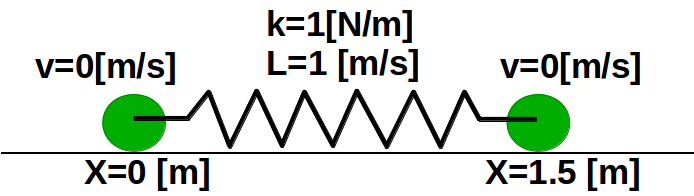
\includegraphics[scale=0.3]{./FigureB.png}
 \caption{Simulación realizada en etapa 2, en la simulación ambas bolas comienzan en reposo una en x=0[mts] y la otra es en x=1.5[mts] ambos con radio 0.1 [mts],
 el resorte efectúa fuerzas según la ley de hooke sobre ambas bolas con stifness = 1 y largo natural 1.}
  \label{etapa2.1}
\end{figure}

Se ha simulado la situación descrita en la figura \ref{etapa2.1}. Con la simulación se obtuvieron el siguiente gráfico.

\begin{figure}[H]
 \centering
 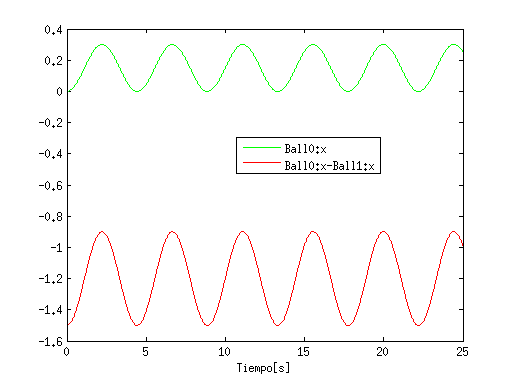
\includegraphics[scale=0.5]{./simulacion_etapa2.png}
 \caption{Resultados simulación etapa 2, en el gráfico se muestran dos diferentes datos en uno la posición de la bola que está inicialmente
 situada en 0 y la otra es la diferencia entre las bolas.}
  \label{etapa1.2}
\end{figure}

  Se observa un comportamiento deseado: ambas bolas oscilan y además su distancia también oscila demostrando que el resorte se contrae y se acercan
  y se expande como se esperaría de la situación ideal presentada.\newline
  
  Además de esta situación se simuló otra situación más con bolas y resortes: dos bolas unidas con un resorte, una de las bolas tiene velocidad inicial
  por lo que el momentum del sistema tiene dirección (así este sistema se ira moviendo al mismo tiempo en que se contrae y se expande) y
  además hay una tercera bola que inicialmente está en reposo y que posteriormente es colisionada por este sistema. Los resultados de este otro
  experimento son los siguientes.
  
  \begin{figure}[H]
 \centering
 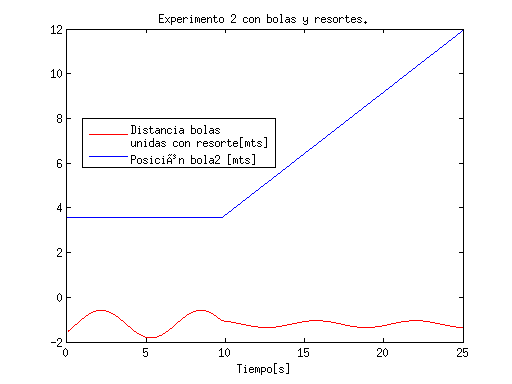
\includegraphics[scale=0.5]{./simulacion_etapa2_experimento2.png}
 \caption{Experimento alternativo etapa2: dos bolas unidas con resorte tienen momentum inicial (dado que una de las bolas tiene velocidad incial) colisionan una tercera bola
 (bola2) que toma parte de la energía del sistema y sale con velocidad constante, luego el sistema al haber perdido momentum oscila con menor amplitud.}
  \label{etapa1.3}
\end{figure}
  
  El resultado es bueno dado que se observa como el sistema entrega parte de su momentum (y su energía) a la bola2 (tercera bola que estaba en reposo).\newline
  
  
 

\end{document}